\documentclass[11pt]{article}
\usepackage{acl2014}
\usepackage{times}
\usepackage{url}
\usepackage{latexsym}
\usepackage{graphicx}
\title{Coconut palms and hand palms: improving similarity ranking by word sense disambiguation}

\author{Anouk Visser \\
  {\tt email} \\\And
  R\'emi de Zoeten \\
  {\tt email} \\}

\date{}

\begin{document}
\maketitle
\begin{abstract}
The abstract will be here.
\end{abstract}

\section{Introduction}

\section{Related Work}
Automatic Word Sense Discrimation by schutze?
Word sense disambiguation is the task of assigning labels to occurrences of ambiguous words. 
Word sense discrimination divides the occurrences of a word in a numb of classes by determining for any towo occurrences whether they belong to the same sense or not. 
\subsection{Word Sense Disambiguation}
\begin{enumerate}
\item Something about the relatedness paper that is really old \cite{relatedness}
\item Something from the survey that gives state of the art about supervised, unsupervised, semi-supervised and knowledge based and how unsupervised is really useful \cite{survey}
\item About analysis \cite{analysis}
\end{enumerate}
\subsection{Word Sense Disambiguation and word vector representations}
\begin{enumerate}
\item Something on word vector representations \cite{word2vec}
\item Problem: nice description in the global paper \cite{global}
\item First and second order clustering, different clustering methods \cite{clustering}
\item Solution: multi-prototype does context and not context \cite{multi}
\item Global paper that can do both, plus new evaluation \cite{global}
\end{enumerate}
Final new thing
Latent meanings \cite{latent}

\section{Training data}
For model training data we used the enwiki8 dataset \cite{enwiki} corpus. For our purposes we filtered the corpus for 

\section{COCONUT}
%COPIED FROM REPORT ULL (SHOULD BE ADJUSTED)
The COCONUT method for disambiguating words is based on two assumptions: 
\begin{enumerate}
\item the meaning of a word is highly dependent on the words it co-occurs with
\item the co-occurring words that define one meaning of a word are more likely to co-occur with each other than two words that define two different meanings of the word
\end{enumerate}

Let $C$ be the set of words that co-occur with $A$, the word we want to disambiguate. COCONUT first constructs and converts the global co-occurrence vectors of the words in $C$ to relatedness vectors. It will then cluster these relatedness vectors in order to determine the two possibly different meanings of $A$. 

\subsection{Co-Occurrence Vectors}
A global co-occurrence vector contains the frequencies indicating how many times two words co-occur, we convert the absolute frequencies in the global co-occurrence vector to a relatedness score. We use the same function for relatedness as \cite{relatedness}:
$$r(x, y) = \frac{f_xy}{f_x+f_y - f_{xy}}$$
where $f_{xy}$ denotes the frequency of $x$ and $y$ occurring together and $f_x$ and $f_y$ denote the frequency of $x$, respectively $y$. 

Words that are not closely related to $A$ do not contribute to either one of the meanings. Therefore, we will discard the words that have a relatedness score with $A$ that falls in the bottom $50\%$ of all relatedness-scores from $C$. The terms that are discarded are considered relevant to all meanings of $A$, we will call this set $R$.

\subsection{Clustering and splitting}
Let the set of co-occurrence vectors from the words in $C$, be called $V$. After applying k-means clustering on the vectors in $V$ we expect to find two cluster centers that represent the two meanings for $A$. Note that we are only interested in describing the two meanings of $A$ using the words in $C$. Therefore, for every vector in $V$ we will discard all words that are not in $C$. The adjusted vectors can now be used to perform k-means clustering. 

The two new co-occurrence vectors for $A$ are initialized with the words in $R$. As the cluster centers define the different meanings of $A$, we can look at the words in each cluster to fill the new co-occurrence vectors for $A$.  

COCONUT will split every word in the corpus in order to find two different meanings (we excluded the 75 most frequent words), but not all words are ambiguous. We expect that words that have two distinct meanings will have a greater cluster distance (i.e. a greater distance between the two meanings) than words that do not. We discard all disambiguations for the words that have a cluster distance that falls in the bottom $50\%$ of all cluster distances.
\begin{figure*}
\center
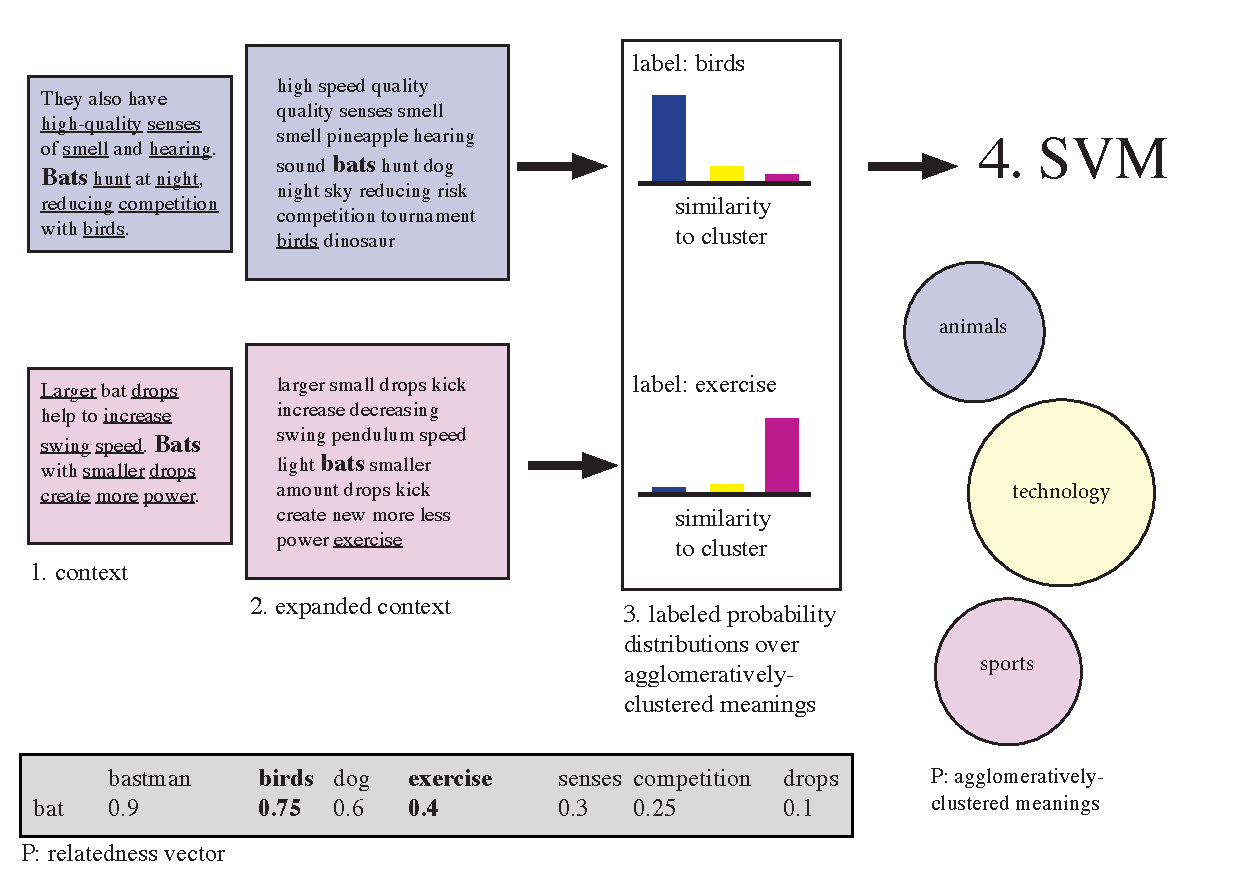
\includegraphics[scale=0.75]{images/palm.pdf}
\caption{The five steps of the PALM algorithm. P: preprocessing, PALM requires agglomeratively-clusterd latent meanings and relatedness vectors for all words in the corpus. 1. Extract every context word $W$ appears in. 2. Expand the context. 3. Choose a label from the expanded context and create a `histogram' over the agglomeratively-clusterd latent meanings for every expanded corpus. 4. Train an SVM on these histograms using the labels.}
\label{palmimg}
\end{figure*}

\section{Agglomerative Clustering}
One way to cluster data is agglomerative clustering. Agglomerative clustering is an iterative bottom up approach to clustering. At the start each data point forms its own cluster and in each iteration the two data points that are closest to each other are merged until there is only a given number of clusters or the smallest inter-cluster distance is larger than a predefined value. Agglomerative clustering can be used to cluster words based on their word vector representation. 




\section{PALM}
In order to disambiguate between multiple meanings of a word, it can be useful to look at the context. PALM is a method for word sense discrimination that trains an SVM for every word that given a context predicts a label that describes the meaning of the word. These labels can be used to relabel a corpus before training a recurrent neural network to obtain multiple vector representations for one word. In this section we describe the PALM method in detail, figure \ref{palmimg} provides an overview of the algorithm. 

\subsection{Choosing the label}
Let $W$ be the word for which we want to train the SVM. PALM starts by extracting all contexts that $W$ appears in. We define `context' as all words within a window around $W$ (in our experiments we looked five words back and five words ahead). Our aim is to assign a label to each of these contexts that describes the sense of the words best, the collection of labels then represent the different sense a word can have. As we have seen in \cite{analysis} underspecified contexts are often observed. In line with our assumption for the COCONUT baseline (i.e. the co-occurring words that define one meaning of a word are more likely to co-occur with each other than two words that define two different meanings of the word) we expand the context by adding the $n$ (in our experiments we set $n=5$) most related words to every word in the context (except for $W$). Finally, a word from the expanded context is selected as a label so that:
$$label = \arg\max_w \frac{r(W, w) + \textit{sim}(W, w)}{2}$$
where $\textit{sim}(W, w)$ denotes the cosine similarity between $W$ and $w$. 

\subsection{Probability distribution over agglomeratively-clustered latent meanings}
For every word in the expanded context we find the similarity to every agglomeratively-clustered latent meaning, creating an $N$ dimensional vector (where $N$ is the number of agglomeratively-clustered latent meanings that were found). These vectors are accumulated and normalized, so that we have one vector for every context. Although the values denote the accumulated similarity of the words from the expanded context to the meanings, we can interpret the vector as a probability distribution over meanings, given the context (when the context and a meaning are very similar, it is very likely that the context imposes this meaning). 

\subsection{Label reduction}
The last step before training the SVM consists of reducing the number of labels. Although including the second-order context by expanding the context radically decreases the number of new labels, there will still be many labels including a number of labels that describe the same sense of $W$. We have implemented a method for label reduction that favors labels that were observed most frequently. We iteratively split the labels into two halves: the upper half (containing labels that were seen most frequently) and the lower half (containing labels that were seen least frequently) and merge a label (and all of its vectors) from the lower half ($w_l$) into a label form the upper half ($w_u$). $w_l$ and $w_u$ are chosen by: 
$$\arg\max_{w_l, w_u} \textit{sim}(w_l, w_u)$$
This process continues until $\textit{sim}(w_l, w_u)$ is below a certain threshold (in our experiments the threshold was $0.5$).
The reordered labelled data can then be used to train an SVM. The SVM can then disambiguate a word by predicting a the most appropriate label given the probability distribution from an expanded context over the agglomeratively-clustered latent meanings. 
%\section{REMI}

\section{Experiments}
%Possible things to evaluate 
%\begin{enumerate}
%\item Is it more beneficial to do PALM with a larger skip size or a larger expansion param?
%\end{enumerate}
\section{Qualitative evaluation}

\section{Quantitative evaluation}

\section{Discussion and future work}
\section{Conclusion}

\bibliographystyle{acl}
\bibliography{cocobib}

\end{document}
